\section{About LaTeX-boilerplate}

\begin{figure}[htbp]
\centering
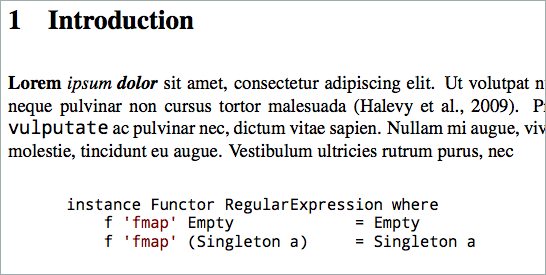
\includegraphics{https://github.com/gbluma/latex-boilerplate/raw/master/screenshot.png}
\caption{Screenshot}
\end{figure}

This project is a placeholder for all of my new LaTeX documents. I've
spent more hours than I care to admit customizing a document format in
the middle or late stages of a project. As deadlines approach I've
rushed to make my document styles look nice and failed. I've learned my
lesson. I'd rather maintain a separate project (this one) that can serve
as a good starting point for new documents and skip that racket.

Note, by default this makescript will convert markdown files into tex
files. Perhaps I haven't drunk enough Kool-aid, but I find TeX to be a
difficult syntax to write in -- except when it offers things that
markdown can't.

Also, I've included a short applescript file called \texttt{focus} which
refreshes the PDF document in Preview.app (on a mac). This hooks into
\texttt{make} so whenever you have new changes just run
\texttt{make test} and you'll see your new changes. I think this is
convenient, but you may disagree.

If you have any recommendations I'd like to hear them.

Thanks.

\section{How to use it?}

Do this and you should have be ready to go.

\begin{verbatim}
cd ~/Documents
git clone git://github.com/gbluma/latex-boilerplate.git newdocument
cd newdocument
make && make open

# do work
make test

# check text for sloppy word usage
make check
\end{verbatim}

By default, the Makefile will build TeX files from any markdown files
that exist in your working directory (prefixed with ``s\_'' indicating
`sections' of your document). I am using Pandoc do handle these
conversions, so if you don't have it or you don't want to use that
workflow, then update the Makefile to bypass \texttt{convert.sh}.

I think Pandoc is a nice addition. It does get me in trouble from time
to time but overall it saves effort. I can use standard Markdown syntax
for 95\% of my writing (bold, italic, code, titles, etc.) and then drop
back to LaTeX for the hard stuff (tables and graphics).
